\section{Architecture and Training}

\subsection{Corruption Rate}

\begin{table}[t]
\begin{subtable}{\linewidth}\centering
{\begin{tabular}{ | m{1cm} | m{1cm} | m{1cm} | m{1cm} | m{1cm} | m{1cm} | m{1cm} | }
  \hline
  & NC & MS & MB & VAR & RET & SL \\
  \hline
  \hline
  100\% & 60.0 & 64.0 & 48.2 & \textbf{37.3} & 54.3 & 26.7 \\
  \hline
  75\% & \textbf{70.4} & \textbf{71.8} & \textbf{51.3} & 34.4 & \textbf{55.1} & \textbf{42.6} \\
  \hline
  50\% & 62.0 & 61.2 & 43.7 & 25.0 & 47.4 & 26.1 \\
  \hline
  25\% & 67.9 & 65.6 & 41.6 & 19.6 & 50.3 & 33.3 \\
  \hline
\end{tabular}}
\caption{Performance of models with different corruption rates.}\label{corruption_rate_table}
\end{subtable}
\newline
\vspace*{5mm}
\newline
\begin{subtable}{\linewidth}\centering
{\begin{tabular}{ | m{3cm} | m{1cm} | m{1cm} | m{1cm} | m{1cm} | m{1cm} | m{1cm} | }
  \hline
  & NC & MS & MB & VAR & RET & SL \\
  \hline
  \hline
  with attention & \textbf{70.4} & \textbf{71.8} & \textbf{51.3} & \textbf{34.4} & \textbf{55.1} & \textbf{42.6} \\
  \hline
  without attention & 0.0 & 0.0 & 0.0 & 0.0 & 0.0 & 0.0 \\
  \hline
  without attention, input reversed & 0.0 & 0.0 & 0.0 & 0.0 & 0.0 & 0.0 \\
  \hline
\end{tabular}}
\caption{Performance of models with or without an attention mechanism.}\label{attention_mechanism_table}
\end{subtable}
\newline
\vspace*{5mm}
\newline
\begin{subtable}{\linewidth}\centering
{\begin{tabular}{ | m{2cm} | m{1cm} | m{1cm} | m{1cm} | m{1cm} | m{1cm} | m{1cm} | }
  \hline
  & NC & MS & MB & VAR & RET & SL \\
  \hline
  \hline
  LSTM & \textbf{70.4} & \textbf{71.8} & \textbf{51.3} & \textbf{34.4} & \textbf{55.1} & \textbf{42.6} \\
  \hline
  GRU & 0.2 & 0.2 & 0.2 & 0.2 & 0.2 & 0.2 \\
  \hline
  vanilla RNN & 0.0 & 0.0 & 0.0 & 0.0 & 0.0 & 0.0 \\
  \hline
\end{tabular}}
\caption{Performance of different RNN types.}\label{rnn_type_table}
\end{subtable}
\caption{Results}
\end{table}

Because the source sequence and target sequence are almost the same and the errors are self-introduced, it is fair to ask what the optimal corruption rate for the input is. To test this the model was trained with four different corruption rates, 100\%, 75\%, 50\% and 25\%. The results can be seen in table \ref{corruption_rate_table}.

For almost all corruptions the model trained with a corruption rate of 75\% posts the best result. The models with lower percentages don't pick up on the errors as well while the model with the 100\% corruption rate lacks the ground truth. In general the model learns to correct all of the introduced errors. It performs especially well when inputting a sequence missing a single semicolon which is of course also the simplest task to solve. However the model is also able to correct the other errors reasonably well. A missing bracket or an incorrect return type are corrected most of the time while the model has a little more trouble correcting a misspelled variable or realigning switched lines. A more detailed analysis for the different error types is given in section \ref{error_analysis}.

What's also interesting to see is how well the model performs on uncorrupted sequences. Even the model with 100\% corruption rate, i.e. which never gets an uncorrupted sequence as input, manages to not introduce any new errors into an uncorrupted sequence most of the time. This indicates that the model obtains some understanding of the input and only corrects where necessary.

\subsection{Attention Mechanism}

\begin{figure}[p]
\centering
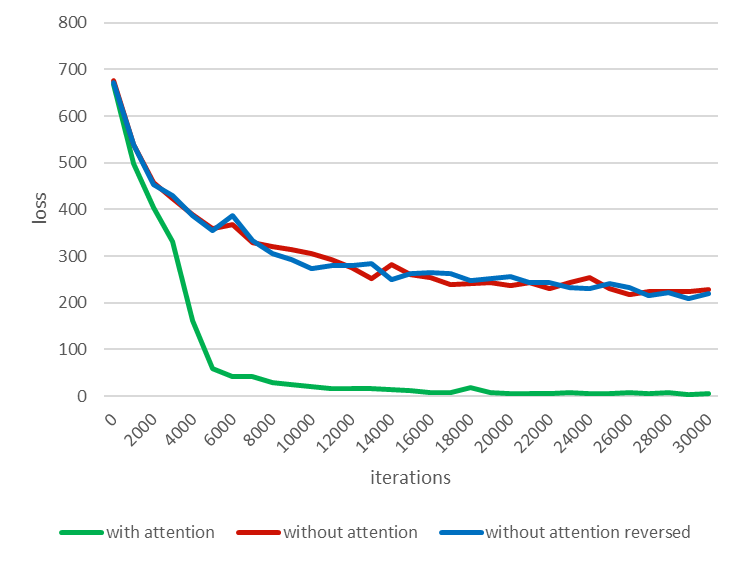
\includegraphics[width=0.9\linewidth]{attention_chart}
\caption{Line chart showing the loss of different models over time.}
\label{attention_chart}
\end{figure}

Of course it can also be asked if the attention mechanism is necessary for the model, after all it increases complexity and training duration. To test this, the model was twice trained without an attention mechanism on top of the decoder, once with the same input the regular model got and once with the input reversed. The reversion of the input is a technique proposed in \cite{seq2seq}, the idea being to introduce more short term dependencies while the average distance of the dependencies stays the same. This is not necessary for the regular model because the attention mechanism allows the model to take a peek of the encoder state at any given timestep.

The experiments revealed the attention mechanism to be an essential part of the model because the models without the mechanism weren't able to solve the given task (see table \ref{attention_mechanism_table}). These models never learnt to repeat the input sequence probably because they couldn't pass all information from the encoder to the decoder in a single vector.

For the first couple of thousand iterations all models learnt roughly the same things, namely the general structure of the desired output. The models would start to begin the output sequence with \texttt{public ...(...)\{} and end it with \texttt{\}<eos>}. In between they added mostly passages they remembered from training. However after about 4,000 iterations the model with the attention mechanism learnt to utilise the mechanism to its full potential and started repeating the input sequence. This resulted in rapid performance improvement. The training loss of the different configurations as a function over iterations can be seen in figure \ref{attention_chart}.

The reversion of the input sequence helped the model to learn a little bit faster and perform a little bit better but overall it made almost no difference. The model was still not able to solve the task.

\subsection{RNN type}

\begin{figure}[p]
\centering
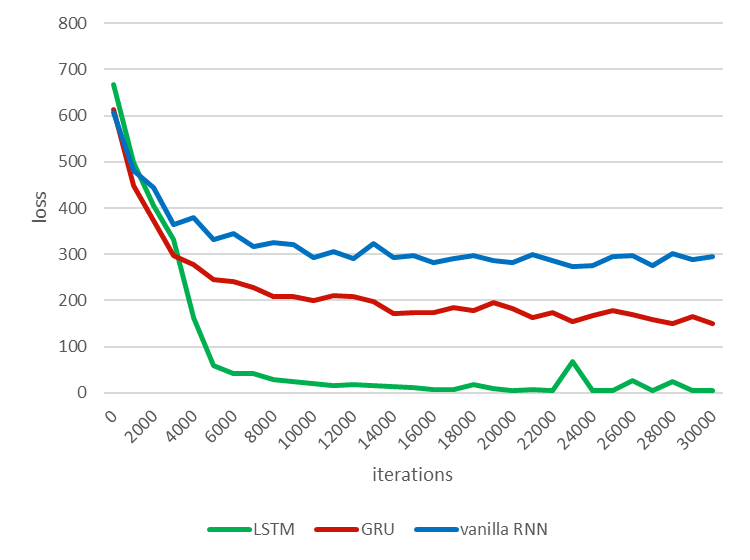
\includegraphics[width=0.9\linewidth]{cell_type_chart}
\caption{Line chart showing the loss of different models over time.}
\label{cell_type_chart}
\end{figure}

In subsection \ref{rnn_types} three types of RNNs were listed: vanilla RNNs, LSTMs and GRUs. To test which type works best for the correction of source code, a model was trained for each RNN type. The training loss of the models as a function over iterations can be seen in figure \ref{cell_type_chart}. The evaluation on the test set can be found in table \ref{rnn_type_table}.

As could be expected the vanilla RNN performed the worst. As explained earlier, these networks struggle to learn long range dependencies and struggle with the problem of vanishing gradients. The vanilla RNN is also the simplest type and thus the one with the least amount of trainable parameters.

More surprising was the performance gap between the GRU and the LSTM, because recent research suggests that these two network types have a comparable performance \cite{lstm_vs_gru}. However similar to the models without the attention mechanism, the GRU network never fully learns to repeat the input sequence. One possible explanation for this are the fewer parameters of the GRU. An LSTM computes three gates at each timestep while also passing a memory vector to the next timestep. A GRU only has two gates and doesn't have a second vector in addition to the hidden state vector. Because the 256 units per layer are on the lower boundary this lack of trainable parameters could prevent the GRU from learning as well as the LSTM.

\section{Error analysis}
\label{error_analysis}

In this section the performance of the model on uncorrupted input and on each of the five corruptions is analysed. For examples from the test set see appendix \ref{showcase}.

\subsection{Uncorrupted}

The model works reasonably well on uncorrupted input with a 70.4\% success rate. However it is still interesting to see, what kind of errors are introduced by the network, i.e. where and why it gets confused. One mistake the model makes repeatedly is a "one-off error". Here the model would output a wrong character whose ASCII encoding is just by one off of the encoding of the correct character. For example sometimes an asterisk whose ASCII encoding is 42 is output while the correct character would be a plus (ASCII encoding 43). If the results of the model are evaluated with a tolerance for these errors (only one off), the accuracy of the model increases to 79.6\%. That's an almost 10\% performance increase and the model should be able to learn to avoid these mistakes with more training.

Another common error is the random switching of lines. An additional 4.8\% of the test set would have been correct if it wasn't for an incorrect line switch. This suggests that the model didn't learn to correct this corruption that well. This problem is elaborated further in subsection \ref{switch_analysis}.

The last thing that was noticeable in the test set was that sometimes the model would get stuck in a loop and output some parts or lines of the input sequence multiple times. This is something that can often be observed in early stages of training which suggests that the model should be able to avoid these mistakes with more training.

\subsection{Missing Semicolon}

The same mistakes from observed on uncorrupted input of course also apply to the correction of corrupted input. The correction of a missing semicolon should be the easiest error to correct. While the correction of a missing semicolon scores already good with 71.8\% accuracy it is also worth to look at the results of an evaluation with the same "one off tolerance" in which case the model is 81.7\% accurate. In addition to that 3.2\% of the time, an error was introduced by an incorrect line switch.

What's also interesting to see is that the output contains the correct number of semicolons in 97.0\% of the time. This means that the missing of a semicolon is detected and corrected nearly every time, there are just new mistakes that are introduced by the model into the output.

\subsection{Missing Brackets}

The main advantage of LSTMs is their ability to remember long range dependencies which should be very useful in inserting missing brackets into the sequence but the test accuracy of 51.3\% seems to contradict this assumption. However a closer look at the results reveal that the task of inserting a missing bracket isn't that trivial. Consider the following example:

\begin{lstlisting}[style=inline]
public int addint a, int b){
  int sum = a + b;
  return sum;
}
\end{lstlisting}

Here the opening brackets between the method name and the parameters was removed. The task for the model is now to not only detect that a bracket is missing but also to find the correct spot to reinsert it which is even more difficult because there is not white space indicating the location of the missing bracket.

To evaluate how many times the missing bracket was detected the test results were evaluated to look if the brackets in the output were balanced, meaning if every opening bracket had a closing counterpart and vice versa. The evaluation showed that the model managed to balance the brackets in 77.2\% of the time. The brackets were also correctly nested 76.9\% of the time which indicates that the model did learn the concept of brackets well.

\subsection{Misspelled Variable}

\begin{figure}[t]
\centering
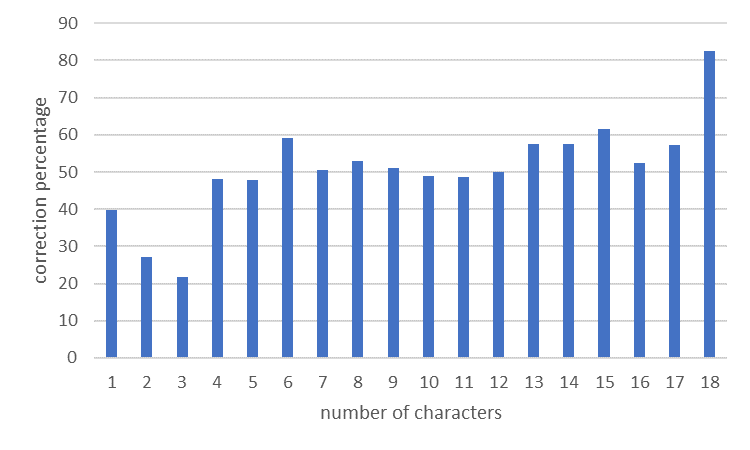
\includegraphics[width=0.9\linewidth]{variables_chart}
\caption{Correction percentage for variables evaluated for different lengths. Only lengths with more than 10 examples were considered.}
\label{variables_chart}
\end{figure}

Including corrected wrong instance: 45.6\%

\subsection{Wrong Return Type}

different percentages

\subsection{Line Switch}
\label{switch_analysis}

\begin{table}[t]
\centering
\begin{tabular}{ | m{1cm} | m{1cm} | m{1cm} | m{1cm} | }
  \hline
  \(\leftrightarrow\) & VD & MI & AS \\
  \hline
  \hline
  VD & - & 53.3 & \textbf{59.3} \\
  \hline
  MI & 0.0 & - & 13.0 \\
  \hline
  AS & 0.0 & 9.8 & - \\
  \hline
\end{tabular}
\caption{VC = Variable Declaration, MI = method invocation, AS = assignment.}
\label{switch_table}
\end{table}
